\begin{textblock*}{3cm}(7.1cm,2cm) % {width}(x, y)
    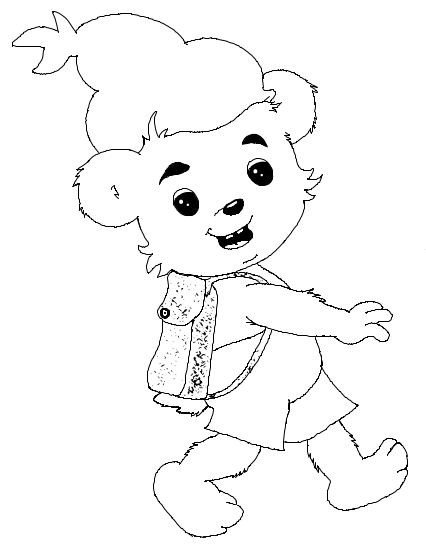
\includegraphics[width=2.4cm]{./bilder/majas-bilder/bamse-1.png}
\end{textblock*}

\begin{textblock*}{3cm}(7.4 cm,5.6cm) % {width}(x, y)
    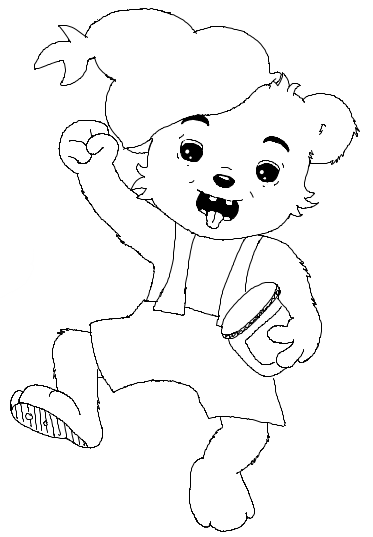
\includegraphics[width=2.2cm]{./bilder/majas-bilder/bamse-2.png}
\end{textblock*}

\begin{textblock*}{3cm}(6.6cm,9.4cm) % {width}(x, y)
    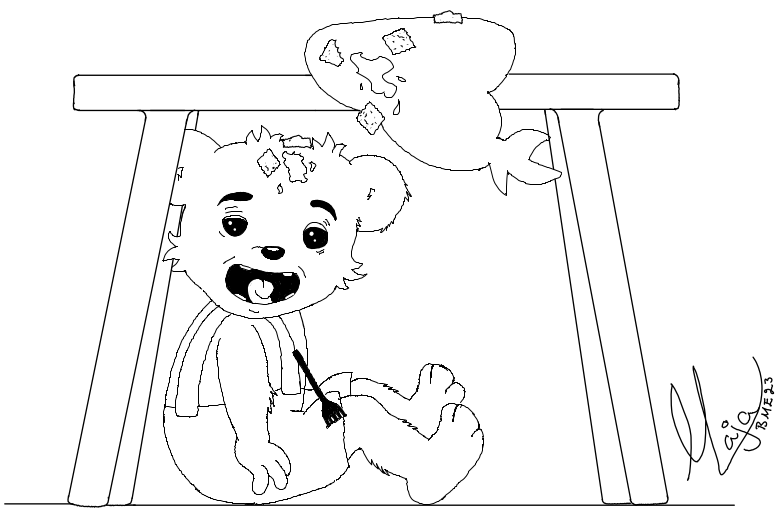
\includegraphics[width=3.6cm]{./bilder/majas-bilder/bamse-3.png}
\end{textblock*}

\subsection*{Jag skall festa} 
\index[alfa]{Jag skall festa}
\index[anfa]{Jag skall festa}
\songinfo{Mel: Bamse\\
Sångarstriden 1987}

\begin{parse lines}[\noindent]{#1\\}
    Jag ska festa, ta det lugnt med spriten,
    ha det roligt utan å va' full
    Inte krypa runt med festeliten,
    ta det varligt för min egen skull

    Först en öl i torra strupen,
    efter det så kommer supen,
    i med vinet, ner med punschen
    Sist en groggbuffé

    Jag är skitfull, däckar först av alla,
    missar festen, men vad gör väl de'?
    Blandar hejdlöst öl och gammal filmjölk,
    kastar upp på bordsdamen breve'!

    Först en öl... 

    Spyan rinner ner för ylleslipsen
    Raviolin torkar i mitt hår
    Vem har lagt mig under matsalsbordet?
    Vems är gaffeln i mitt högra lår?
\end{parse lines}

\vissteduatt{Innan pandemin skrev alla programmeringstentor på papper?}
\newpage


\begin{textblock*}{3cm}(5.6cm,3.3cm) % {width}(x, y)
    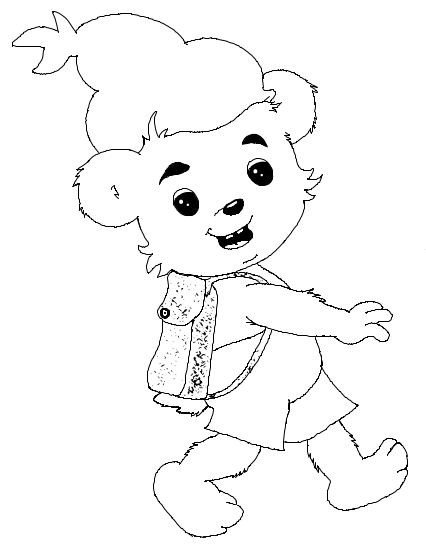
\includegraphics[width=2.4cm]{./bilder/majas-bilder/bamse-1.png}
\end{textblock*}

\begin{textblock*}{3cm}(8cm,4.5cm) % {width}(x, y)
    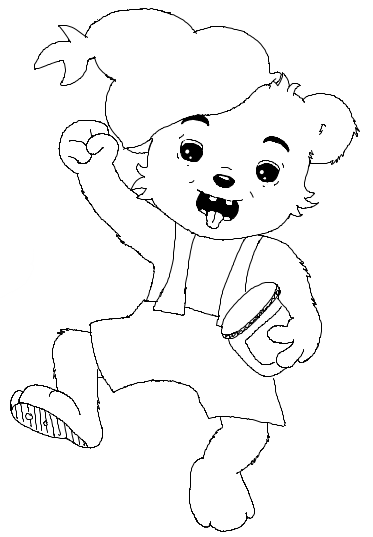
\includegraphics[width=2.2cm]{./bilder/majas-bilder/bamse-2.png}
\end{textblock*}

\begin{textblock*}{3cm}(6.6cm,7.6cm) % {width}(x, y)
    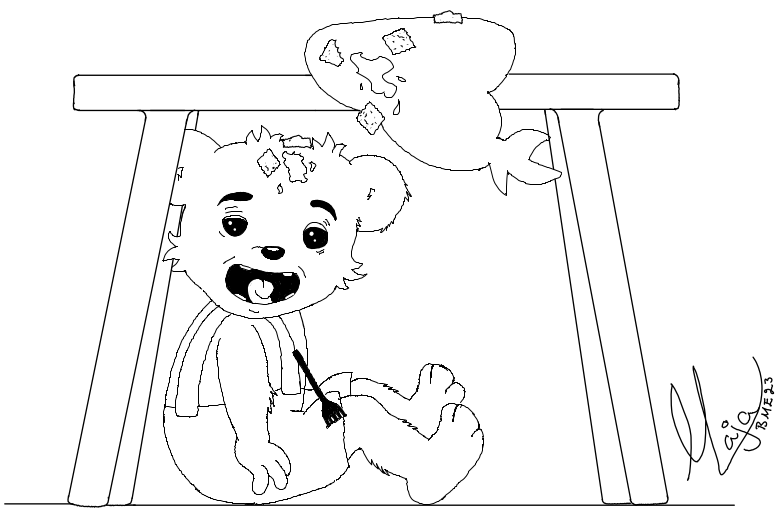
\includegraphics[width=3.6cm]{./bilder/majas-bilder/bamse-3.png}
\end{textblock*}

\subsection*{Jag skall festa} 
\index[alfa]{Jag skall festa}
\index[anfa]{Jag skall festa}
\songinfo{Mel: Bamse\\
Sångarstriden 1987}

\begin{parse lines}[\noindent]{#1\\}
    Jag ska festa, ta det lugnt med spriten,
    ha det roligt utan å va' full
    Inte krypa runt med festeliten,
    ta det varligt för min egen skull

    Först en öl i torra strupen,
    efter det så kommer supen,
    i med vinet, ner med punschen
    Sist en groggbuffé

    Jag är skitfull, däckar först av alla,
    missar festen, men vad gör väl de'?
    Blandar hejdlöst öl och gammal filmjölk,
    kastar upp på bordsdamen breve'!

    Först en öl... 

    Spyan rinner ner för ylleslipsen
    Raviolin torkar i mitt hår
    Vem har lagt mig under matsalsbordet?
    Vems är gaffeln i mitt högra lår?
\end{parse lines}


\vissteduatt{Innan pandemin skrev alla programmeringstentor på papper?}
\newpage


\begin{textblock*}{3cm}(6cm,7.8cm) % {width}(x, y)
    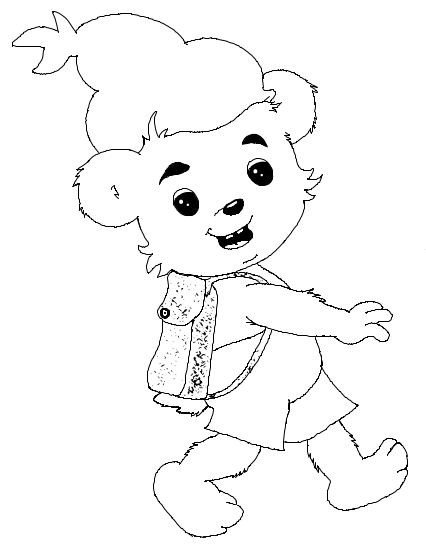
\includegraphics[width=2.4cm]{./bilder/majas-bilder/bamse-1.png}
\end{textblock*}

\begin{textblock*}{3cm}(8.3cm,9.5cm) % {width}(x, y)
    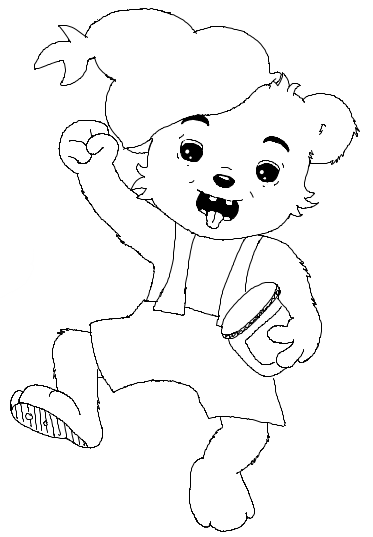
\includegraphics[width=2.2cm]{./bilder/majas-bilder/bamse-2.png}
\end{textblock*}

\begin{textblock*}{3cm}(4.7cm,11.1cm) % {width}(x, y)
    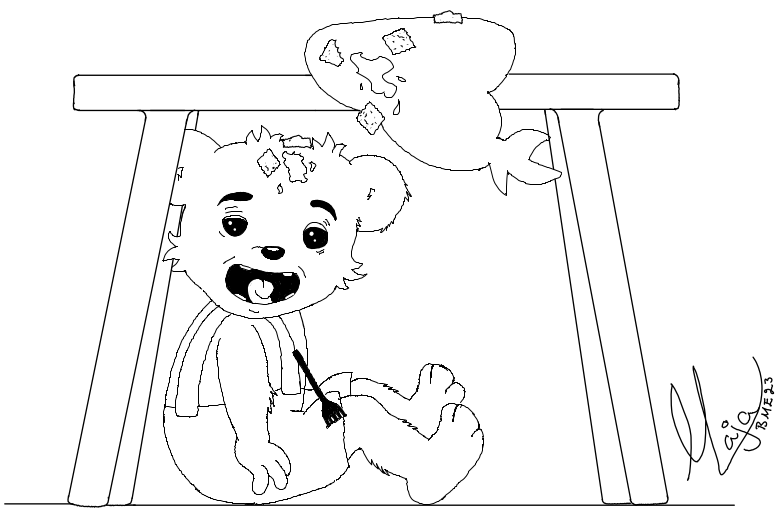
\includegraphics[width=3.6cm]{./bilder/majas-bilder/bamse-3.png}
\end{textblock*}

\subsection*{Jag skall festa} 
\index[alfa]{Jag skall festa}
\index[anfa]{Jag skall festa}
\songinfo{Mel: Bamse\\
Sångarstriden 1987}

\begin{parse lines}[\noindent]{#1\\}
    Jag ska festa, ta det lugnt med spriten,
    ha det roligt utan å va' full
    Inte krypa runt med festeliten,
    ta det varligt för min egen skull

    Först en öl i torra strupen,
    efter det så kommer supen,
    i med vinet, ner med punschen
    Sist en groggbuffé

    Jag är skitfull, däckar först av alla,
    missar festen, men vad gör väl de'?
    Blandar hejdlöst öl och gammal filmjölk,
    kastar upp på bordsdamen breve'!

    Först en öl... 

    Spyan rinner ner för ylleslipsen
    Raviolin torkar i mitt hår
    Vem har lagt mig under matsalsbordet?
    Vems är gaffeln i mitt högra lår?
\end{parse lines}


\vissteduatt{Innan pandemin skrev alla programmeringstentor på papper?}
\newpage


\begin{textblock*}{3cm}(5.5cm,3.2cm) % {width}(x, y)
    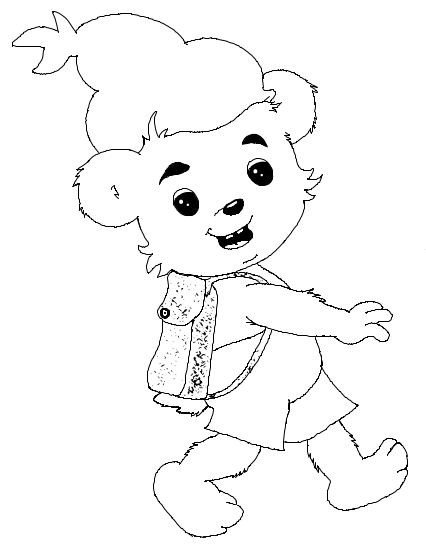
\includegraphics[width=2.8cm]{./bilder/majas-bilder/bamse-1.png}
\end{textblock*}

\begin{textblock*}{3cm}(7.6cm,6.7cm) % {width}(x, y)
    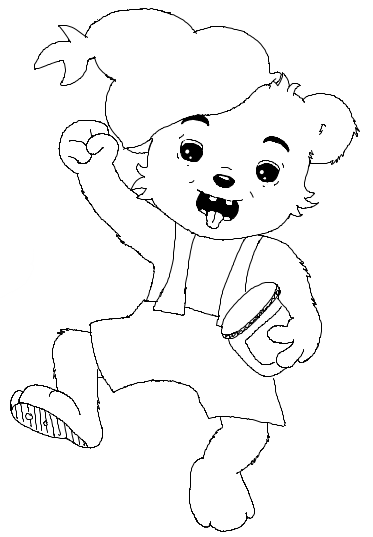
\includegraphics[width=2.6cm]{./bilder/majas-bilder/bamse-2.png}
\end{textblock*}

\begin{textblock*}{3cm}(5.6cm,10.2cm) % {width}(x, y)
    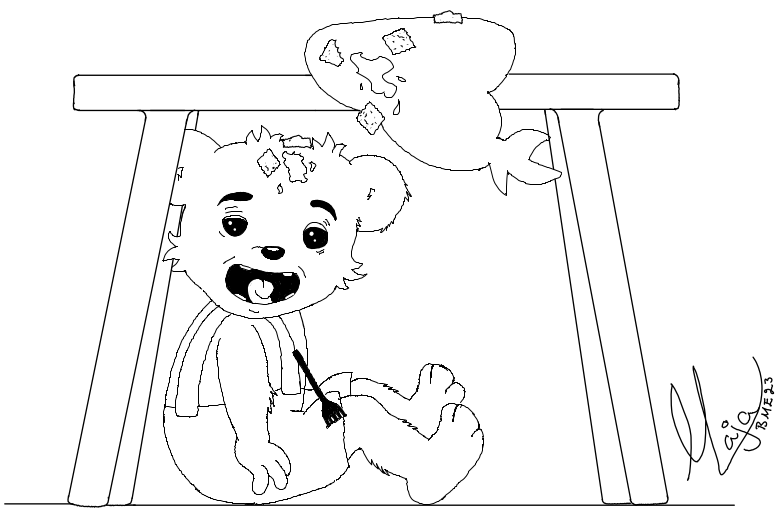
\includegraphics[width=4.9cm]{./bilder/majas-bilder/bamse-3.png}
\end{textblock*}

\subsection*{Jag skall festa} 
\index[alfa]{Jag skall festa}
\index[anfa]{Jag skall festa}
\songinfo{Mel: Bamse\\
Sångarstriden 1987}

\begin{parse lines}[\noindent]{#1\\}
    Jag ska festa, ta det lugnt med spriten,
    ha det roligt utan å va' full
    Inte krypa runt med festeliten,
    ta det varligt för min egen skull

    Först en öl i torra strupen,
    efter det så kommer supen,
    i med vinet, ner med punschen
    Sist en groggbuffé

    Jag är skitfull, däckar först av alla,
    missar festen, men vad gör väl de'?
    Blandar hejdlöst öl och gammal filmjölk,
    kastar upp på bordsdamen breve'!

    Först en öl... 

    Spyan rinner ner för ylleslipsen
    Raviolin torkar i mitt hår
    Vem har lagt mig under matsalsbordet?
    Vems är gaffeln i mitt högra lår?
\end{parse lines}


\vissteduatt{Innan pandemin skrev alla programmeringstentor på papper?}
\newpage


\begin{textblock*}{3cm}(7.5cm,1.5cm) % {width}(x, y)
    %\scalebox{-1}[1]{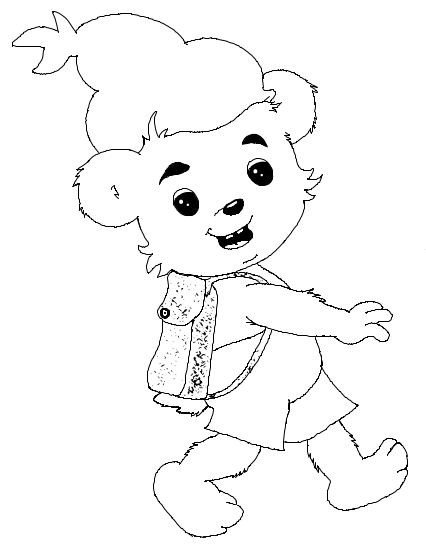
\includegraphics[width=2.4cm]{./bilder/majas-bilder/bamse-1.png}}
    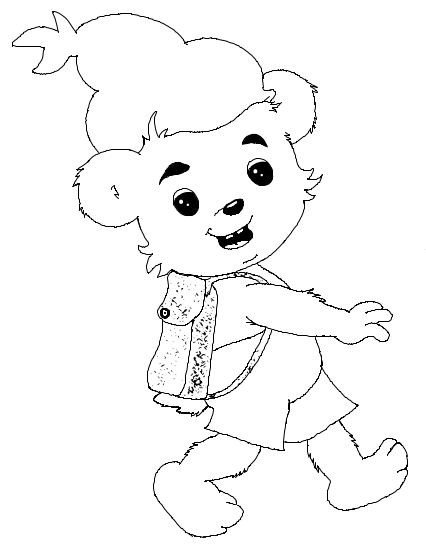
\includegraphics[width=2.4cm]{./bilder/majas-bilder/bamse-1.png}
\end{textblock*}

\begin{textblock*}{3cm}(6cm, 4.1cm) % {width}(x, y)
    \scalebox{-1}[1]{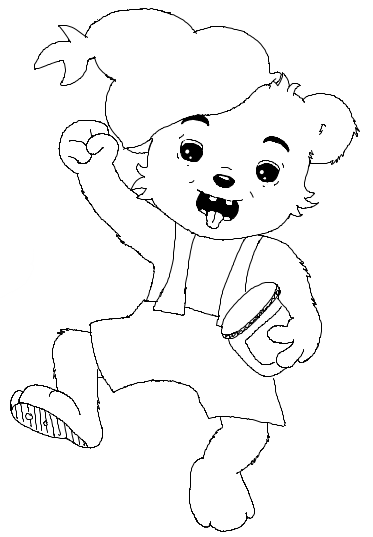
\includegraphics[width=2.2cm]{./bilder/majas-bilder/bamse-2.png}}
\end{textblock*}

\begin{textblock*}{3cm}(6.6cm,7.6cm) % {width}(x, y)
    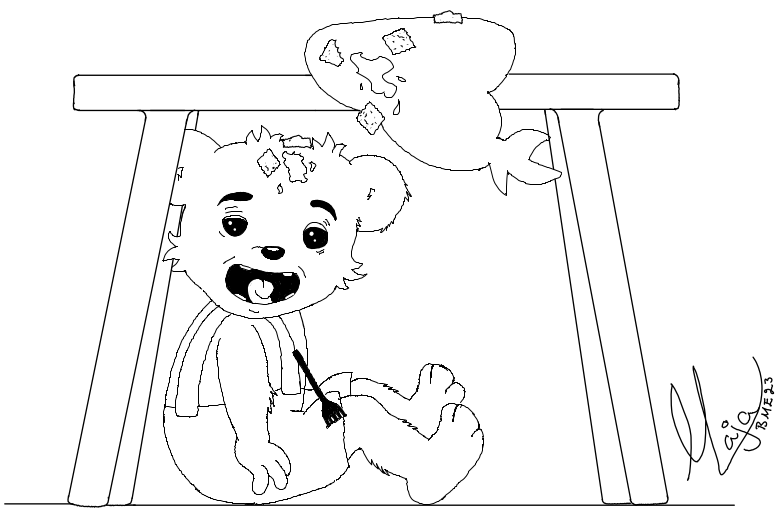
\includegraphics[width=3.6cm]{./bilder/majas-bilder/bamse-3.png}
\end{textblock*}

\subsection*{Jag skall festa} 
\index[alfa]{Jag skall festa}
\index[anfa]{Jag skall festa}
\songinfo{Mel: Bamse\\
Sångarstriden 1987}

\begin{parse lines}[\noindent]{#1\\}
    Jag ska festa, ta det lugnt med spriten,
    ha det roligt utan å va' full
    Inte krypa runt med festeliten,
    ta det varligt för min egen skull

    Först en öl i torra strupen,
    efter det så kommer supen,
    i med vinet, ner med punschen
    Sist en groggbuffé

    Jag är skitfull, däckar först av alla,
    missar festen, men vad gör väl de'?
    Blandar hejdlöst öl och gammal filmjölk,
    kastar upp på bordsdamen breve'!

    Först en öl... 

    Spyan rinner ner för ylleslipsen
    Raviolin torkar i mitt hår
    Vem har lagt mig under matsalsbordet?
    Vems är gaffeln i mitt högra lår?
\end{parse lines}


\vissteduatt{Innan pandemin skrev alla programmeringstentor på papper?}
\newpage

\begin{textblock*}{3cm}(5.5cm,3.3cm) % {width}(x, y)
    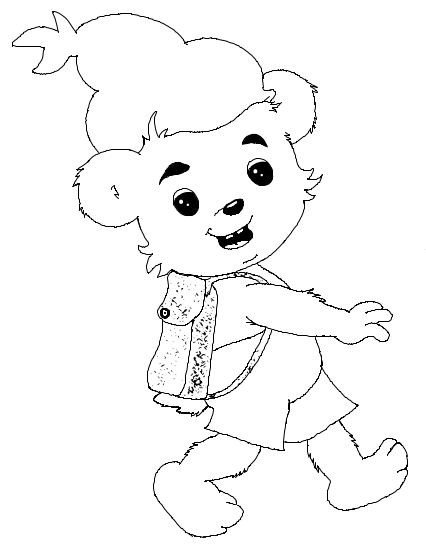
\includegraphics[width=2.4cm]{./bilder/majas-bilder/bamse-1.png}
\end{textblock*}

\begin{textblock*}{3cm}(7.8cm,4.6cm) % {width}(x, y)
    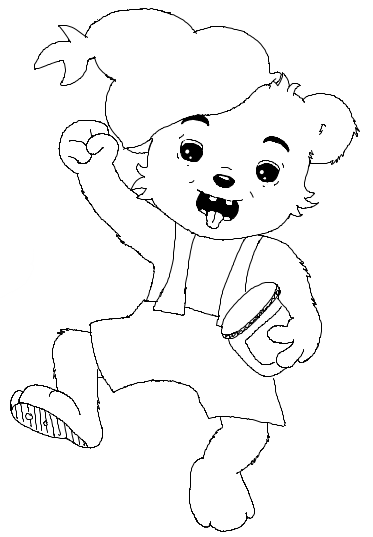
\includegraphics[width=2.2cm]{./bilder/majas-bilder/bamse-2.png}
\end{textblock*}

\begin{textblock*}{3cm}(6 cm,7.6cm) % {width}(x, y)
    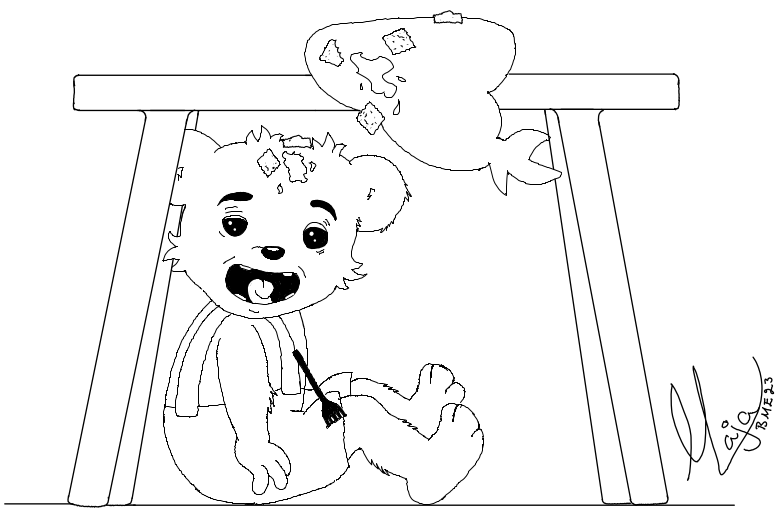
\includegraphics[width=3.6cm]{./bilder/majas-bilder/bamse-3.png}
\end{textblock*}

\subsection*{Jag skall festa} 
\index[alfa]{Jag skall festa}
\index[anfa]{Jag skall festa}
\songinfo{Mel: Bamse\\
Sångarstriden 1987}

\begin{parse lines}[\noindent]{#1\\}
    Jag ska festa, ta det lugnt med spriten,
    ha det roligt utan å va' full
    Inte krypa runt med festeliten,
    ta det varligt för min egen skull

    Först en öl i torra strupen,
    efter det så kommer supen,
    i med vinet, ner med punschen
    Sist en groggbuffé

    Jag är skitfull, däckar först av alla,
    missar festen, men vad gör väl de'?
    Blandar hejdlöst öl och gammal filmjölk,
    kastar upp på bordsdamen breve'!

    Först en öl... 

    Spyan rinner ner för ylleslipsen
    Raviolin torkar i mitt hår
    Vem har lagt mig under matsalsbordet?
    Vems är gaffeln i mitt högra lår?
\end{parse lines}


\vissteduatt{Innan pandemin skrev alla programmeringstentor på papper?}
\newpage
